%% This is the main file and you use this file to organize your assignment.

\documentclass[a4paper]{article}
\usepackage[margin=3cm]{geometry} 	   % Choose your margin here. 
\usepackage{amsmath}
\usepackage{parskip}
\usepackage{graphicx}
\usepackage{caption}
\usepackage{subcaption}

\newcommand{\figref}[1]{\figurename~\ref{#1}}

\let\endtitlepage\relax						% Begin the text immidiately after the title page. Optional
\setlength{\parindent}{0cm}				% Start paragraph without indent. Optional


%Macros
\newcommand\bb[1]{\mathbf{#1}}
\newcommand\bs[1]{\boldsymbol{#1}}

%Todos with overview of todos in \listoftodos
\usepackage{xargs}                      % Use more than one optional parameter in a new commands
\usepackage[pdftex,dvipsnames]{xcolor}  % Coloured text etc.
% 
\usepackage[colorinlistoftodos,prependcaption,textsize=tiny]{todonotes}
\newcommandx{\unsure}[2][1=]{\todo[linecolor=red,backgroundcolor=red!25,bordercolor=red,#1]{#2}}
\newcommandx{\change}[2][1=]{\todo[linecolor=blue,backgroundcolor=blue!25,bordercolor=blue,#1]{#2}}
\newcommandx{\info}[2][1=]{\todo[linecolor=OliveGreen,backgroundcolor=OliveGreen!25,bordercolor=OliveGreen,#1]{#2}}
\newcommandx{\improvement}[2][1=]{\todo[linecolor=Plum,backgroundcolor=Plum!25,bordercolor=Plum,#1]{#2}}
\newcommandx{\thiswillnotshow}[2][1=]{\todo[disable,#1]{#2}}

\begin{document}

\begin{titlepage}
\begin{center}
\Large TTK4190 Guidance and Control of Vehicles \\
\vspace{10pt}
\Large Assignment 1 \\
\vspace{10pt}
\large Written Fall 2017 by Alex Danielsen and Daniel Nakken
\end{center}
\end{titlepage}


%Obs! Macros are used in order to simplify typing. While this is usually bad practice when others are meant to read your code,
%this latex code was only meant to be read by two people agreeing to use macros in order to save time and simplify.

\section*{Problem 1 - Attitude Control of Satellite}
\todo[inline]{Write in an overall understanding of the assignment problem here. What are we doing in this assignment? What are we achieving? What are we learning? What is it the professor and student assistants wants us to have understood from all of this?}
\listoftodos[List of things that need to be done before turn in:]

\subsection*{Problem 1.1} 
Equation (1) from the assignment is:
\begin{equation}
\label{eq:dynamics}
	\begin{aligned}
		\dot{\mathbf{q}} = \mathbf{T}_q (\mathbf{q} ) \boldsymbol{\omega} \\
		\mathbf{I}_{CG} \dot{\boldsymbol{\omega}} - \mathbf{S} (\mathbf{I}_{CG} \boldsymbol{\omega} ) \boldsymbol{\omega} & =  \boldsymbol{\tau}
	\end{aligned}	
\end{equation}
We find the equilibrium point of  $\bb{q}$ \eqref{eq:dynamics} where the label makes sure that the correct equation number is used. If you want to write an equation directly in the text (outside of the equation environment), use: $\dot{\mathbf{q}} = \mathbf{T}_q (\mathbf{q} ) \boldsymbol{\omega}$. % You have to use the dollar sign to write math symbols within a text.

A matrix (and an equation without equation number) can be created as: 
\begin{equation*}	% The star indicates that you don't want to give this equation a number. Normally used if you don't refer to the equation.
	\mathbf{A} = 
	\begin{bmatrix}
		a & b & c \\ d & e & f \\ g & h & i
	\end{bmatrix}
\end{equation*}

\subsection*{Problem 1.2}
Answer Problem 1.2 here. Bold words can be written as \textbf{something bold}. It is also possible to create a new section level:
\subsubsection*{Inner Section 1}
\emph{text..}

\subsubsection*{Inner Section 2}
...

\subsection*{Problem 1.3}
Answer Problem 1.3 here. Equation (2) from the assignment can be written as: 
\begin{equation}
  \label{eq:tau}
  \mathbf{\tau} = -\mathbf{K}_d \boldsymbol{\omega} - k_p \boldsymbol{\epsilon}
\end{equation}

\subsection*{Problem 1.4}
The quaternion error can be written as
 \begin{equation}
	 \tilde{\mathbf{q}} := \left[
	 \begin{array}{c}
		 \tilde{\eta} \\
		 \tilde{\epsilon}
	 \end{array}
	 \right] = \bar{\mathbf{q}}_d \otimes \mathbf{q} 
 \end{equation}

\subsection*{Problem 1.5}
...

\subsection*{Problem 1.6}
...

\subsection*{Problem 1.7}
The Lyapunov function can be written as 
 \begin{equation}
	 V = \frac{1}{2} \tilde{\boldsymbol{\omega}}^{\top} \mathbf{I}_{CG}\tilde{\boldsymbol{\omega}} + 2 k_p (1-\tilde{\eta})
 \end{equation}

\subsection*{Problem 1.8}
...

% Note that \mathbf can be used for bold letters in math mode (within equations and dollar signs). \boldsymbol can be used to get bold greek letters.  	% Use "\include" instead of "\input" if you want the section to start on a new page. "problem1" is a tex file included at this location in the document. It is possible to answer the whole assignment in the main file (paste everything from "problem1.tex" and "problem2.tex" here), but that restricts the readability. Therefore, one file is created for each problem.
\section*{Problem 2 - Underwater Vehicles}
Answer Problem 2 in this file. 
\subsection*{Problem 2.1}
Answer problem 2.1 here. The Greek letters for sideslip, crab and course are $\beta_r$, $\beta$ and $\chi$, respectively. The Greek letter for the flight-path angle is $\gamma$.

\subsection*{Problem 2.2}
Answer Problem 2.2 here. The body-fixed velocities can be written as
\begin{equation}
\label{eq:velocity}
	\begin{bmatrix}
		u \\
		v \\
		w
	\end{bmatrix}
	= 
	\begin{bmatrix}
		U \cos( \omega t)\\
		U \sin(\omega t)\\
		0	
	\end{bmatrix}
\end{equation}

\subsection*{Problem 2.3}
Answer Problem 2.3 here.

\subsection*{Problem 2.4}
Answer Problem 2.4 here. Figures can be inserted as:
\begin{figure}[ht]
	\centering
	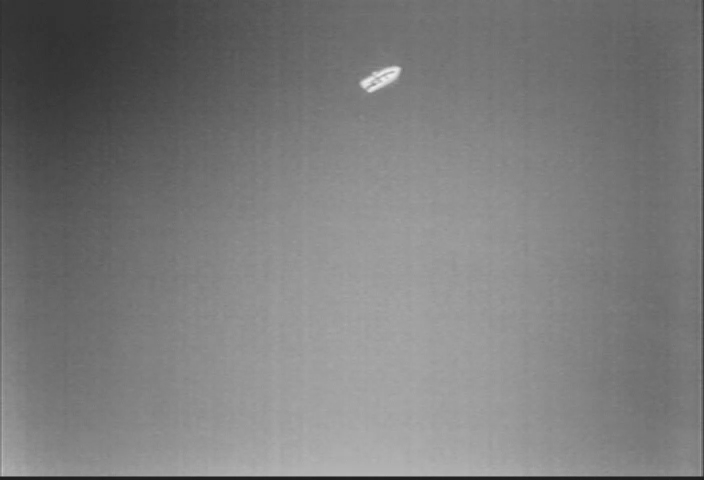
\includegraphics[width=0.7\textwidth]{fig1} % Filename is "fig1.png" and must be located in the same folder as this file. If you have a folder containing all the figures you can use "Figures/fig 1" as long as the "Figures" folder is placed in the same folder as this file.
	\caption{Figure of something useful.}
	\label{fig:fig1}
\end{figure}

You can now refer to this figure as \figref{fig:fig1}. You can also insert figures side-by-side:
\begin{figure}[ht]
	\centering
	\begin{subfigure}[b]{0.45\textwidth}
		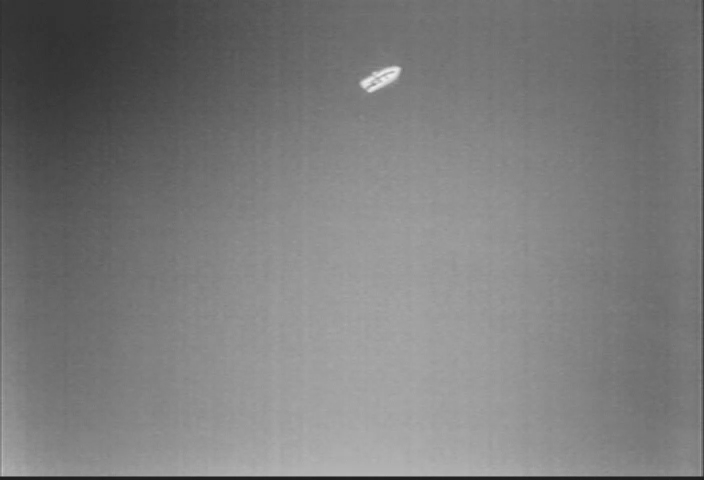
\includegraphics[width=\textwidth]{fig1}
		\caption{caption..}
		\label{fig:2a}
	\end{subfigure}
	~ %add desired spacing between images, e. g. ~, \quad, \qquad, \hfill etc. 
	%(or a blank line to force the subfigure onto a new line)
	\begin{subfigure}[b]{0.45\textwidth}
		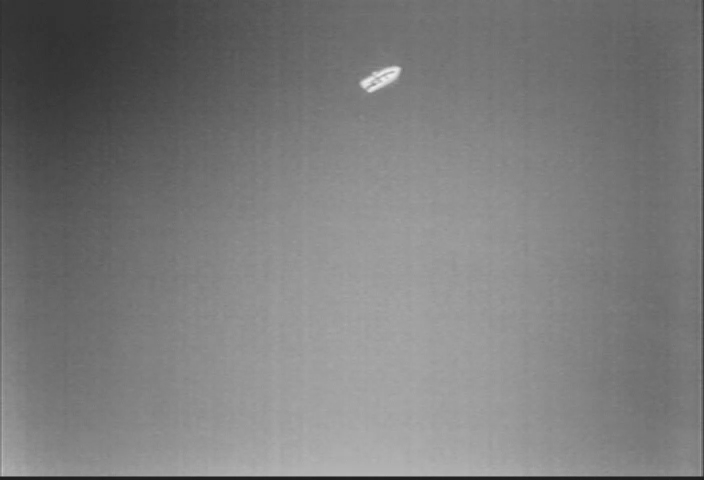
\includegraphics[width=\textwidth]{fig1}
		\caption{caption..}
		\label{fig:2b}
	\end{subfigure}
	\begin{subfigure}[b]{0.45\textwidth}
		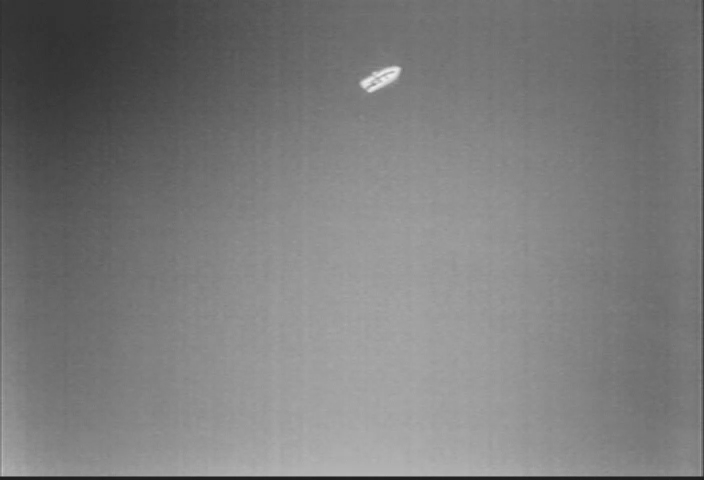
\includegraphics[width=\textwidth]{fig1}
		\caption{caption..}
		\label{fig:2c}
	\end{subfigure}
	\begin{subfigure}[b]{0.45\textwidth}
		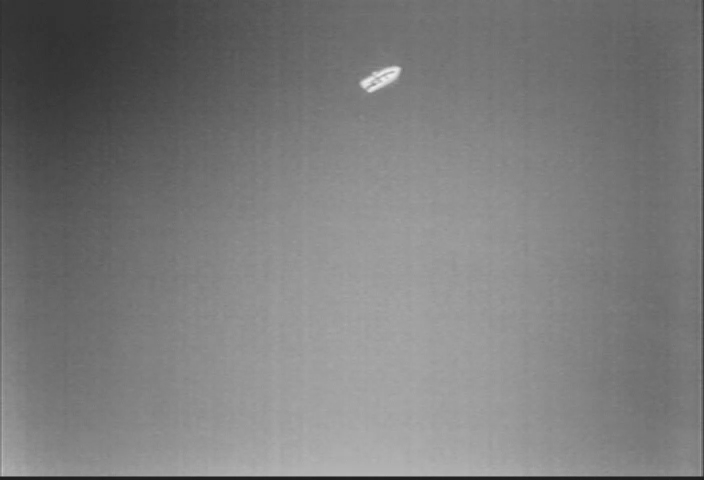
\includegraphics[width=\textwidth]{fig1}
		\caption{caption..}
		\label{fig:2d}
	\end{subfigure}		
	\caption{Caption for all figures}\label{fig:2}
\end{figure}

\subsection*{Problem 2.5}
The Nomoto model can be written as
\begin{equation}
	\frac{r}{\delta} (s) = \frac{K}{Ts+1}
\end{equation}
and the equations for the roll and pitch rate as
\begin{equation}
\begin{aligned}
	&\dot{p} + 2\zeta_p\omega_p p + \omega_p^2 \phi = 0\\
	&\dot{q} + 2\zeta_q\omega_q q + \omega_q^2 \theta = 0
\end{aligned}
\end{equation}

\subsection*{Problem 2.6}
References can be placed in the bibliography.bib and referred to as \cite{Fossen2011} and \cite{Fjellstad1994857}.

 
\bibliographystyle{IEEEtran}
\bibliography{bibliography.bib}

\end{document}